%%%%%%%%%%%%%%%%%%%%%%%%%%%%%%%%%%%%%%%%%%%%%%%%%%%%%%%%%%%
% if you want to add fontawesome package
% you need to compile the tex file with LuaLaTeX
%
%%%%%%%%%%%%%%%%%%%%%%%%%%%%%%%%%%%%%%%%%%%%%%%%%%%%%%%%%%%
%
% File needed in the smae pakge :
% 1. friggeri-cv.cls  -> src: https://www.sharelatex.com/project/58fb3afaf6e52d83685040bd
% 2. Lato-Hairline.ttf  -> src: 
% 3. pgfsys-luatex.def -> src: https://sourceforge.net/p/pgf/bugs/_discuss/thread/44f8dcf2/9dc8/attachment/pgfsys-luatex.def 

%
%%%%%%%%%%%%%%%%%%%%%%%%%%%%%%%%%%%%%%%%%%%%%%%%%%%%%%%%%%%
%
%	The Head
%
\documentclass[]{friggeri-cv}

%%% pakges to import auto  %%%
\usepackage[utf8]{inputenc} %
\usepackage{afterpage}
\usepackage{hyperref}
\usepackage{color}
\usepackage{xcolor}
\usepackage{smartdiagram}
\usepackage{fontspec}
%
%
%
\usepackage{metalogo}
%%%%\usepackage{dtklogos}
\usepackage[utf8]{inputenc}
\usepackage{tikz}
\usepackage{multicol}


%%%
\usetikzlibrary{mindmap,shadows}

%%%
\hypersetup{
    pdftitle={},
    pdfauthor={},
    pdfsubject={},
    pdfkeywords={},
    colorlinks=false,           % no link border color
    allbordercolors=white       % white border color for all
}

%%%
\smartdiagramset{
    bubble center node font = \footnotesize,
    bubble node font = \footnotesize,
    % specifies the minimum size of the bubble center node
    bubble center node size = 2.5cm,
    %  specifies the minimum size of the bubbles
    bubble node size = 1cm,
    % specifies which is the distance among the bubble center node and the other bubbles
    distance center/other bubbles = 0.5cm,
    % sets the distance from the text to the border of the bubble center node
    distance text center bubble = 0.5cm,
    % set center bubble color
    bubble center node color = pblue,
    % define the list of colors usable in the diagram
    set color list = {lightgray, materialcyan, materialorange, green, orange, materialteal, materialamber, materialindigo, materialgreen, materiallime},
    % sets the opacity at which the bubbles are shown
    bubble fill opacity = 0.6,
    % sets the opacity at which the bubble text is shown
    bubble text opacity = 0.5,
}
%%%

%%% FOR C# symbol
\newfontface\lserif{Liberation Serif}

\newcommand{\Csh}{C{\lserif\#}}

%%%%%%%%%%%%%%%%%%%%%%%%%%%%%%%%%%%%%%%%%%%%%%%%%%%%%%%%%%%
%
%	The Body
%
\begin{document}
%% 1. Header
\header{Albarudy }{ Salem}{Computer Engineer}
     
% 2. Fake text to add separator      
\fcolorbox{white}{gray}{\parbox{\dimexpr\textwidth-2\fboxsep-2\fboxrule}{%
.....}}

% 3.  In the LEFT aside, each new line forces a line break
\begin{aside}
	% 3.1. my Foto
	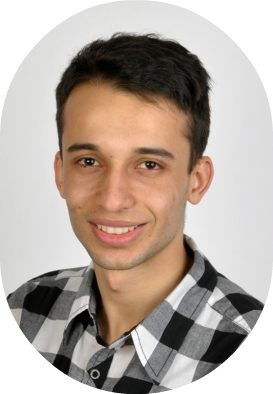
\includegraphics[scale=0.3]{img/rounded_corners-1.png}		
	\section{Address}
		Poland, Kielce
    	~
  	\section{Tel \& Skype}
    	+48 881-550-520
   		salem.albarudy
    	~
  	\section{Mail}
    	\href{mailto:saljan93@live.com}{\textbf{saljan93@}\\live.com}
    	~
  	\section{Web \& Git}
    	\href{https://github.com/SalAlba}{github.com/SalAlba}
	    \href{https://bitbucket.org/saljan}{bitbucket.org/saljan}
    	~
	\section{OS Preference}
    \textbf{GNU/Linux}
\includegraphics[scale=0.40]{img/5stars.png}
    \textbf{Windows}
\includegraphics[scale=0.40]{img/4stars.png}
    ~
  \section{Languages}
    \textbf{Polish}
\includegraphics[scale=0.40]{img/5stars.png}
    \textbf{Arabic}
\includegraphics[scale=0.40]{img/5stars.png}
    \textbf{English}
\includegraphics[scale=0.40]{img/3stars.png}
    ~
  \section{Places Lived}
    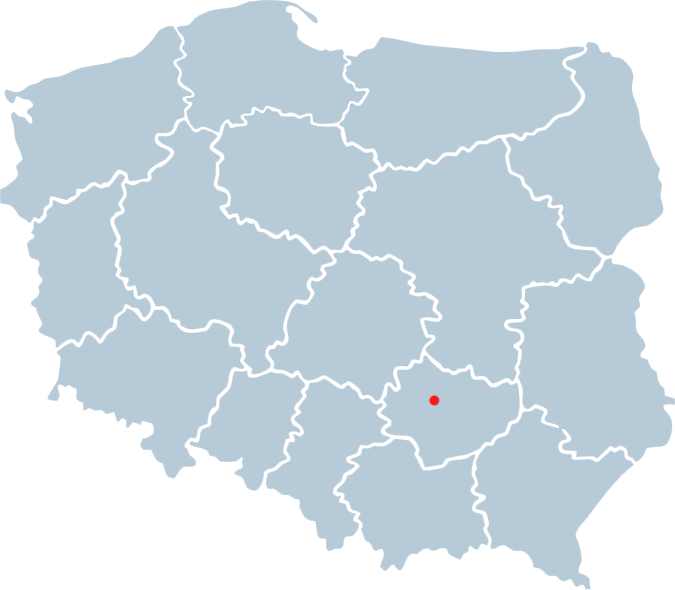
\includegraphics[scale=0.15]{img/pl-1.png}
    ~
\end{aside}

% 4.
\section{Education}
\begin{entrylist}
  \entry
  	%% Date  %%
    {2017 - Now}
    %% Title  %%
    {Master's Degree in Computer Engineering}
    %% Right Title  %%
	{\href{http://tu.kielce.pl/}{ 
\includegraphics[scale=0.25]{img/psk_fb_logo_180px.png} Kielce University Of Technology } }
	%% Content  %%
    {Working on Project, allow to build app using visual components.\\}
  \entry
    {2013 - 2017}
    {Bachelor's Degree in Computer Engineering}
   	{\href{http://tu.kielce.pl/}{
\includegraphics[scale=0.25]{img/psk_fb_logo_180px.png} Kielce University Of Technology } }
	{The aim of the thesis project is to develop a web application and its service, used to conduct educational courses. Besides the typical tasks associated with service users expect that the work will be implemented advanced mechanics course management of content. For backend will be used perform JEE (database can be any). Frontend will be in AngularJS.\\}
\end{entrylist}


%% 5.
\section{Experience}
\begin{entrylist}
  \entry
    {07/2015 -  10/2016}
    {  Web Developer}
    {\href{http://jagiello.solutions/}{ 
\includegraphics[]{img/favicon.png} Jagiello Solutions } }
    {  }  
\end{entrylist}

%% 6.
\section{Skills}
\begin{multicols}{2}
%% COL-1
\smartdiagramset{
  planet size=2cm, 
  distance planet-text=0.1,
  distance planet-satellite=2.5cm,
  /tikz/connection planet satellite/.append style={<-}
} 
\smartdiagram[constellation diagram]{
  JSE/JEE,JPA,Hibernate,EJB3,JAX-RS,Jersey,JSF,Primefaces,JavaFX
}

%%
\columnbreak
%%


%% COL-2
\smartdiagram[bubble diagram]{
        \textbf{JS},
        \textbf{P5.JS},
        \textbf{Bootstrap},
        \textbf{AngularJS},
        \textbf{Other\vspace{3mm}},
        \textbf{JQuery},
        \textbf{PHP}\\\textbf{CakePHP. 2.*.},
        \textbf{HTML/CSS}
}
\end{multicols}

Additional
\begin{itemize}
  \item Android 
  \item  C/\Csh{}
  \item UML 
\end{itemize}


%%
\begin{flushleft}
	\emph{January, 2017}
\end{flushleft}
\begin{flushright}
	\emph{Salem Albarudy}
\end{flushright}

\end{document}